\subsection{Non-Photorealistic Rendering shading styles}
As previously said, the goal of \cite{referencePaper} is to render 3D objects \textit{without any constraint} on the
choice of material or illumination, while taking into consideration the way of Geometry-based Shading technique that \textit{enhances the lighting} at each surface point. \newline
To achieve this, the authors of \cite{referencePaper} demonstrated their approach with three different \textbf{non-photorealistic shading styles}: \textit{Blinn-Phong Shading}, \textit{Cartoon shading} and \textit{Gooch} Shading. For each of those styles, they \textbf{adapted} their technique by choosing properly an \textbf{intensity mapping} function $\delta$ to be used in the reflected radiance equation.
\pagebreak
\subsubsection{Enhanced Blinn-Phong Shading implementation}
In the context of non-photorealistic rendering, it is common to make use of \textit{simple shading models} such as Blinn-Phong shading model. \newline
Geometry-based shading technique can alter surface shading to enhance surface fine-scale \textbf{geometric details} in a non-photorealistic manner. This process is performed by incorporating enhanced surface normal and surface curvature measure into Blinn-Phong.
\newline
As \textbf{intensity mapping} function \cite{referencePaper} choosed $\delta_j$ = $\rho_j$, where j $\in$ \{ a, d, s \} iterates over the components of Blinn-Phong's shading models: ambient, diffuse and specular. \newline
With this approach, using a single light, the lightning equation becomes:
\begin{equation}
	L_r(x,\omega_o) = \sum_j \rho_j(\omega_o,l) \mathcal{G}_j(x,\omega_o,l) L_j(l)
\end{equation}
In this equation, l is the direction of the light source at point x, $L_j$ corresponds to the light intensity of each component, $\rho_a$ = 1, $\rho_d(l)$ = $(n'\cdot  l)$, $\rho_d(s)$ = $(n'\cdot  r)^f$; \newline
$n'(x)$ is the \textbf{enhanced surface normal}, r is the reflection direction, f is the shininess parameter and $\mathcal{G}_j(x,\omega_o,l)$ corresponds to the \textbf{Curvature-based Reflectance Scaling Function}. \newline
In particular, $\mathcal{G}_j$ is computed as:
\begin{equation}
	\mathcal{G}_j(\delta, P) = \frac{\delta}{e^P (1-\delta) + \delta}\quad\mathrm{where}\quad  P_{\lambda,\alpha}(k) = pow(\lambda |k|, \alpha)
\end{equation}
In this equation, $P_{\lambda,\alpha}$ is the \textbf{curvature mapping} function; its magnitute and strength are controlled using two parameters $(\lambda,\alpha)$; $\delta$ corresponds to the previously declared \textbf{intesity mapping} function.\newline
Code-wise, I started from Blinn-Phong implementation, already present in \textbf{lecture03a} repository, and modified it as we can see in \textbf{Code \ref{code:blinn-phong-enhanced}}, introducing all the previously listed functions. \newline
\begin{lstlisting}[language=C++, caption=Enhanced Blinn-Phong subroutine and Curvature-Based Reflectance scaling function implemented in fragment shader,label={code:blinn-phong-enhanced}]
	
	
	
	// Curvature-Based Reflectance Scaling Function
	float Lr(float curvature_value, float delta)
	{
		// We apply the curvature mapping function that uses lambda and alpha parameters to apply non-linear mapping
		float P = pow (lambda * abs(curvature_value), alpha);
		// Uses as intensity mapping function the second parameter, delta
		// This function maps intensity mapping and curvature mapping functions in the reflectance radiance equation
		// This aims to correlate the reflected lightning intensity to surface curvature
		float G = delta / ( exp(P) * ( 1 - delta ) + delta );
		return G;
	}













	// a subroutine for the Enhanced Blinn-Phong model using Shape Depiction Enhancement based on local Geometry 
	subroutine(ill_model)
	vec3 EnhancedBlinnPhong()
	{
		// Computing the mask for Unsharp Masking
		vec3 mask = vNormal - vSMNormal;
		// calculating enhanced Normal using the Unsharp Masking technique. This is defined, in the reference paper, in equation 6 of chapter 4.2.2
		vec3 eNormal = vNormal + lambda * mask;
		// normalization of the per-fragment enhanced normal 
		vec3 N_I = normalize(eNormal);
		// calculating curvature value using enhanced normal
		float curvature_value = curvature(N_I);
		// Implementing equation 12 of chapter 6.1 of the reference paper. I calculate the Curvature-Based Reflectance Scaling factor for each of the Blinn-Phong components. NOTE: Reference paper use the costant 1 as rho_a component for ambient
		float rhoA = 1;
		float G_a = Lr(curvature_value, rhoA);  
		// ambient component can be calculated at this point
		vec3 color = Ka * G_a * ambientColor;
		// normalization of the per-fragment light incidence direction
		vec3 L = normalize(lightDir.xyz);
		// Lambert coefficient
		float rhoD = max(dot(L,N_I), 0.0);
		// if the lambert coefficient is positive, then I can calculate the specular component
		if(rhoD > 0.0)
		{
			// This is the Curvature-Based Reflectance Scaling factor for the diffuse component. NOTE: Reference paper use the lambertian coefficient as rho_d for diffuse
			float G_d = Lr(curvature_value, rhoD); 
			// the view vector has been calculated in the vertex shader, already negated to have direction from the mesh to the camera
			vec3 V = normalize( vViewPosition );
			// in the Blinn-Phong model we do not use the reflection vector, but the half vector
			vec3 H = normalize(L + V);
			// we use H to calculate the specular component
			float specAngle = max(dot(H, N_I), 0.0);
			// shininess application to the specular component
			float rhoS = pow(specAngle, shininess);
			// This is the Curvature-Based Reflectance Scaling factor for the specular component. NOTE: Reference paper use the lambertian coefficient as rho_s for specular
			float G_s = Lr(curvature_value, rhoS);
			// We add diffusive and specular components to the final color using our Curvature-Based factors
			color += vec3( Kd * G_d * diffuseColor +
			Ks * G_s * specularColor);
		}
		return color;
	}

\end{lstlisting}
A Comparison between standard Blinn-Phong and Enhanced Blinn-Phong using Geometry-based shading is showed in \textbf{Figure \ref{fig:blinn_comparison}} that use two subroutines created in the project.
\pagebreak
\begin{figure}[h]
	\centering
	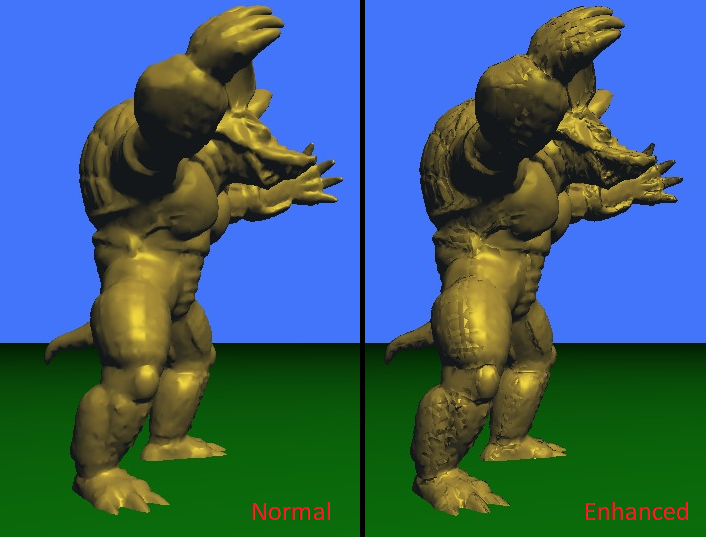
\includegraphics[width=0.8\textwidth]{Images/blinn_comparison.png}
	\caption{Comparison between standard Blinn-Phong and Enhanced Blinn-Phong using Geometry-based shading}
	\label{fig:blinn_comparison}
\end{figure}

\subsubsection{Enhanced Cartoon/Cel Shading implementation}
Lorem ipsum dolor sit amet, consectetur adipiscing elit. Aliquam fringilla fringilla dui id vehicula. Vestibulum aliquet, dui non viverra cursus, odio felis laoreet justo, ultricies blandit massa elit id lacus. Donec est lorem, aliquet ac gravida ac, egestas in elit. Sed sed ultrices tellus. Sed placerat nibh vel leo elementum, at aliquet turpis auctor. Etiam volutpat est risus, sit amet vehicula justo molestie sit amet. Donec fermentum libero in risus lobortis pellentesque. Sed dapibus, leo in congue dapibus, risus risus congue dolor, ac convallis lectus magna placerat ligula. Nam at turpis nisi. In scelerisque, libero vel laoreet tristique, est nunc maximus ipsum, non laoreet orci lorem ut dui. Cras vel est at ex congue congue sit amet id lectus. Nullam in tortor elementum, tempus eros vel, sagittis diam. Curabitur ultrices est nec est rhoncus malesuada. Mauris rhoncus nulla in ligula congue rhoncus. Suspendisse aliquet pellentesque lacus, nec varius neque sagittis et.
\subsubsection{Enhanced Gooch Shading implementation}
Lorem ipsum dolor sit amet, consectetur adipiscing elit. Aliquam fringilla fringilla dui id vehicula. Vestibulum aliquet, dui non viverra cursus, odio felis laoreet justo, ultricies blandit massa elit id lacus. Donec est lorem, aliquet ac gravida ac, egestas in elit. Sed sed ultrices tellus. Sed placerat nibh vel leo elementum, at aliquet turpis auctor. Etiam volutpat est risus, sit amet vehicula justo molestie sit amet. Donec fermentum libero in risus lobortis pellentesque. Sed dapibus, leo in congue dapibus, risus risus congue dolor, ac convallis lectus magna placerat ligula. Nam at turpis nisi. In scelerisque, libero vel laoreet tristique, est nunc maximus ipsum, non laoreet orci lorem ut dui. Cras vel est at ex congue congue sit amet id lectus. Nullam in tortor elementum, tempus eros vel, sagittis diam. Curabitur ultrices est nec est rhoncus malesuada. Mauris rhoncus nulla in ligula congue rhoncus. Suspendisse aliquet pellentesque lacus, nec varius neque sagittis et.